\section{Theory}
\label{chap:Theory}

\subsection{Linear Regression Theory}
\label{chap:Linear Regression Theory}

\quad \, Linear regression analysis performs a significant purpose in statistical modelling and is broadly applied nowadays. This technique is a linear approach to modelling the relationship between a response or dependent variable and explanatory or independent variables. In the case of only one explanatory variable, this is called a single linear regression, and for more than 2, we have a denominated multiple linear regression.\\

These relationships between variables are modelled using linear predictor functions, in other words, combinations of a set of unknown coefficients and known explanatory variables resulting in the response variables. Once we have a bunch of data observations, this is easy to infer the unknown coefficients from the techniques, and then we will end up with a model which can predict a response from any explanatory data.\\

Consider that we have a data-set that shows the values of an observation $\textbf{z} = [z_0, z_1, .., z_{n-1}]$, the dependent response from a set of explanatory values $\textbf{x} = [x_0, x_1, .., x_{n-1}]$. Since we do not know how to explain $\textbf{z}$ in terms of $\textbf{x}$, in other words, we do not have any known function $\textbf{f}(*)$ underlying this case, but there is somehow a correlation between $\textbf{z}$ and $\textbf{x}$, and no multicollinearity among the values of $x_i$, then a linear regression can be formed.\\

From these assumptions, it is usual to understand that $\textbf{z}$ and $\textbf{x}$ have a linear relationship between each other, and we can create a parametrization of the unknown function $\textbf{f}(*)$ from, for instance, a polynomial of degree ($p$), such that:\\

\begin{equation}
\label{eq1}
z = z(x) \rightarrow z(x_i)=z_i=\tilde{z}_i+\epsilon_i=\sum_{j=0}^{p}\beta_j x_i^j + \epsilon_i
\end{equation}\\

For that, we needed to introduce a coefficient $\beta_i$ and an independently and normally distributed noise $\epsilon_i$, which are the foundation of the linear regression model, hence these raises the set of the following equations:\\

$$z_0&=\beta_0+\beta_1x_0^1+\beta_2x_0^2+\dots+\beta_{n-1}x_0^{p}+\epsilon_0$$
$$z_1&=\beta_0+\beta_1x_1^1+\beta_2x_1^2+\dots+\beta_{n-1}x_1^{p}+\epsilon_1$$
$$z_2&=\beta_0+\beta_1x_2^1+\beta_2x_2^2+\dots+\beta_{n-1}x_2^{p}+\epsilon_2$$
$$&\vdots $$
$$z_{n-1}&=\beta_0+\beta_1x_{n-1}^1+\beta_2x_{n-1}^2+\dots+\beta_{n-1}x_{p}^{n-1}+\epsilon_{n-1}$$\\

We now consider $z_i$ as a stochastic values which approximates to the real $z$. Besides, the interpretation of $z_i$ is the expectation of a response $z_i$ given a explanatory observation $x_i$, such that:  $z_i=E[z_i|x_i]$.\\

Then, we re-writing everything as vectors and matrices:\\

$$\textbf{z} = [z_0,z_1, z_2,..., z_{n-1}]^T$$
$$\boldsymbol{\beta} = [\beta_0,\beta_1, \beta_2,\dots, \beta_{p-1}]^T$$
$$\boldsymbol{\epsilon} = [\epsilon_0,\epsilon_1, \epsilon_2,\dots, \epsilon_{n-1}]^T$$

$$\boldsymbol{X}=
\begin{bmatrix} 
1& x_{0}^1 &x_{0}^2& \dots &x_{0}^{p} \\
1& x_{1}^1 &x_{1}^2& \dots &x_{1}^{p} \\
1& x_{2}^1 &x_{2}^2& \dots &x_{2}^{p} \\                      
\vdots& \vdots &\vdots& \cdots &\vdots \\
1& x_{n-1}^1 &x_{n-1}^2& \dots &x_{n-1}^{p} \\
\end{bmatrix}$$ \\

\noindent where $\textbf{X} \in \mathbb{R}^{n \times p}$ is a design matrix from $p$ quantity of explanatory variables (columns) with $n$ number of samples (rows). \\

Finally, equation (\ref{eq1}) can be written as:\\

\begin{equation}
\label{eq2}
\boldsymbol{z} = \boldsymbol{\tilde{z}} + \boldsymbol{\epsilon} = \boldsymbol{X\beta} + \boldsymbol{\epsilon}
\end{equation}\\

\subsubsection{Ordinary least squares}
\label{chap:Ordinary least squares}

\qquad \, Ordinary least of squares is a technique of estimating the unknown coefficient $\beta$ from the model.\\

We pick a set of $\beta=(\beta_0, \beta_1, ..., \beta_p)^T$ from the minimization of the residual sum of squares: $RSS(\beta)=\sum^N_{i=1}(z_i-f(x_i))^2=\sum^N_{i=1}(z_i-\beta_0-\sum^p_{j=1}x_{ij}\beta_j)^2$, where the training observations $(x_i, z_i)$ are a representation of independent random draws from their population, or $z_i$'s are conditionally independent given inputs $x_i$. \\

Denote $\textbf{X}$ as the $N\times(p+1)$ matrix where each row is an input vector, and $\textbf{z}$ is the (N-vector,) of outputs. Then, $RSS(\beta)=(\textbf{z}-\textbf{X}\beta)^T(\textbf{z}-\textbf{X}\beta)$ is a quadratic function with $(p+1)$ coefficients. Assuming that $\textbf{X}$ has full column rank, $\textbf{X}^T\textbf{X}$ is positive definite and differentiating with respect to $\beta$, we obtain:\\

\begin{equation}
\label{eq3}
\hat{\beta}=E[\beta]=(\textbf{X}^T\textbf{X})^{-1}\textbf{X}^T\textbf{z}
\end{equation}\\

\noindent where $\hat{\beta}$ is the optimal beta, or minimized beta.\\

Since we got the minimized $\hat{\beta}=(\textbf{X}^T\textbf{X})^{-1}\textbf{X}^T\textbf{z}$, then the predicted values are\\

\begin{equation}
\label{eq4}
\tilde{\textbf{z}}=E[y]=\textbf{X}\hat{\beta}=\textbf{X}(\textbf{X}^T\textbf{X})^{-1}\textbf{X}^T\textbf{z}
\end{equation}\\

\noindent where it is explained as the projection of $\textbf{z}$ onto the column space of $\textbf{X}$.\\

\subsubsection{Confidence Interval of the coefficients $\beta$}
\label{chap:Confidence Interval of the coefficients beta}

\qquad \, Assume that the observations $z_i$ are uncorrelated and have constant variance $\sigma^2$, and that the $x_i$ are fixed. Then, the variance-covariance matrix of the least square coefficient estimates is given by: \\

\begin{equation}
\label{eq5}
Var[\hat{\beta}]=(\textbf{X}^T\textbf{X})^{-1}\sigma^2
\end{equation}\\

Where the variance $\sigma^2$ can be estimate by $\hat{\sigma}^2=\frac{1}{N-p-1}\sum^N_{i=1}(z_i-\hat{z}_i)^2$. The $(N-p-1)$ makes the $\hat{\sigma}^2$ an unbiased estimate of $\sigma^2$ by $E[\hat{\sigma}^2]=\sigma^2$.\\

Then, the confidence interval for $\beta$ is\\

\begin{equation}
\label{eq6}
(\hat{\beta}_j-Z_{1-\alpha}(\textbf{X}^T\textbf{X})^{-1}\sigma^2, \hat{\beta}_j+ Z_{1-\alpha}(\textbf{X}^T\textbf{X})^{-1}\sigma^2)
\end{equation}\\

\subsubsection{Ridge Regression}
\label{chap:Ridge Regression}

\quad \, The OLS technique has a low bias but a large variance. It also treats all parameters with the same weight, not considering that some predictors may be more important than others. Then, Ridge and Lasso take place.\\

To improve the accuracy of a model, we can reduce or increase some of the coefficients, so-called regularization. Ridge regression is a technique that shrinks the coefficients, some of then turning to zero, by attributing a penalty to their size.\\

We introduce the tuning parameter $\lambda>=0$ that is the amount of shrinkage. Then, the cost function will be:\\

$$C(\boldsymbol{\beta}) = (\boldsymbol{z} - \boldsymbol{X\beta})^T(\boldsymbol{z} - \boldsymbol{X\beta}) + \lambda \boldsymbol{\beta}^T\boldsymbol{\beta}$$\\

\noindent where its penalty is $||\boldsymbol{\beta}||_2^2 = \boldsymbol{\beta}^T\boldsymbol{\beta}$.\\

From it's derivative with respect to $\beta$, we end up with:\\

\begin{equation}
\label{eq7}
\boldsymbol{\hat\beta} = ( \boldsymbol{X}^T\boldsymbol{X} + \lambda \boldsymbol{I} )^{-1} \boldsymbol{X}^T \boldsymbol{z}
\end{equation}\\

\noindent and the outputs $\boldsymbol{\tilde{z}}$ for a given  $\boldsymbol{X}$ is:\\

\begin{equation}
\label{eq8}
\boldsymbol{\tilde{z}} = \boldsymbol{X\beta} = \boldsymbol{X}(\boldsymbol{X}^T\boldsymbol{X}  + \lambda \boldsymbol{I})^{-1}\boldsymbol{X}^T
\end{equation}\\

Note that $\lambda=0$ will results to the OLS.\\

\subsubsection{Lasso Regression}
\label{chap:Lasso Regression}

\quad \, Another regression technique is called Lasso Regression, or Least Absolute Shrinkage and Selection Operator. Its cost function is:\\

$$C(\boldsymbol{\beta}) = (\boldsymbol{y} - \boldsymbol{X}\beta)^T(\boldsymbol{y} - \boldsymbol{X}\beta) + \lambda \sqrt{\boldsymbol{\beta}^T\boldsymbol{\beta}}$$\\

\noindent where its penalty/regularization is $||\boldsymbol{\beta}||_1 = \sqrt{\boldsymbol{\beta}^T\boldsymbol{\beta}}$.\\

It turns out that this penalty transforms the equation into a non-linear form, and then there is no similar linear algebraic solution for $\beta$ as OLS and Ridge. Instead, we use gradient descent to minimize the cost function.\\

\subsection{Machine Learning pre-processing methods}
\label{chap:Machine Learning pre-processing methods}
\subsubsection{Splitting data-set}
\label{chap:Splitting data-set}

\quad \, Typically, a pre-processing step needs to be done before fitting and predicting the data in a Linear Regression model. Many techniques could be applied here, but we first split the data using the sci-kit learn function \href{https://scikit-learn.org/stable/modules/generated/sklearn.model_selection.train_test_split.html}{train\_test\_split(X, z, test\_size=0.2, random\_state=10)}. This function is the most basic model selection procedure where divides a single dataset of X and z into four different blocks, X\_train, X\_test, z\_train, and z\_test, for training and testing purposes. The training sets fit and build the Linear regression model, and the testing sets are for using this built model on unknown values of X\_test for predicting and evaluating the accuracy performance. This model selection is necessary because we can not accurately assess the predictions' accuracy using only data that the predicting model already knows.\\

Therefore, first, one trains the model with the X\_train and z\_train sets and then test this same model using other sets X\_test and z\_test to generate proper measures for the predictions.\\

\subsubsection{Scaling data-set}
\label{chap:Scaling data-set}

\quad \, Another important step, which provides relevant benefits for the linear regression model's accuracy measures, is scaling. This method standardizes and transforms the values of X\_train and X\_test in order to avoid outliers values that can negatively impact the accuracy of the model.\\

The formula for standardization is: $Z = (x - u) / s$,\\

\noindent where: $x$ is each element in a column of X\_train[:, C], $u$ is the mean of all elements in a column of X\_train[:, C], $s$ is the standard deviation of all elements in a column of X\_train, $Z$ is the standardized value of $x$.\\

To do that, we use another sci-kit function called \href{https://scikit-learn.org/stable/modules/generated/sklearn.preprocessing.StandardScaler.html}{StandardScaler}.\\

\subsection{Accuracy measurements}
\label{chap:Accuracy measurements}

\subsubsection{Mean Squared Error}
\label{chap:Mean Squared Error}

\quad \, The first accuracy measure called Mean Squared Error (MSE), which estimates the average of the errors' squares, is given by the following formula:\\

\begin{equation}
\label{MSE-Function}
MSE(\hat{z},\hat{\tilde{z}}) = \frac{1}{n}
\sum_{i=0}^{n-1}(z_i-\tilde{z}_i)^2,
\end{equation}\\

Since the MSE measures the average squared difference between the predicted values and the real value, it is always non-negative, and values closer to zero are desirable.\\

The function is present in the file \href{https://github.com/fabiorodp/UiO-FYS-STK4155/blob/master/Project1/package/accuracies.py}{accuracies.py} in our \href{https://github.com/fabiorodp/UiO-FYS-STK4155/tree/master/Project1/package}{package/} directory.\\

\subsubsection{R2-score}
\label{chap:R2-score}

\quad \, In its turn, the coefficient of determination, or also called r-squared or r2-score, is the rate of variation of a dependent variable (z), which is explained by the independent variables (X), given by the formula:\\

\begin{equation}
\label{R2-Function}
R^2(\hat{z}, \tilde{\hat{z}}) = 1 - \frac{\sum_{i=0}^{n - 1} (z_i - \tilde{z}_i)^2}{\sum_{i=0}^{n - 1} (z_i - \bar{z})^2},
\end{equation}\\

Since r2-score is a rate, its values are up to 1, which 1 indicates the perfect score of the model's accuracy; in other words, it means that the explanatory variables explain 100 percent of the response variable.\\

The function is present in the file \href{https://github.com/fabiorodp/UiO-FYS-STK4155/blob/master/Project1/package/accuracies.py}{accuracies.py} in our \href{https://github.com/fabiorodp/UiO-FYS-STK4155/tree/master/Project1/package}{package/} directory.\\

\subsubsection{Bias-variance trade-off} \\
\label{chap:Bias-variance trade-off}

\quad \, The bias-variance trade-offs play an essential role in Machine Learning when assessing the predicting model's accuracy. \\

Bias is the measure of the distance between our estimate from the real target value. Higher bias tends to underestimate/under-fit the data because it oversimplifies the training. \\

Variance measures the sensitivities of the model. Typically, it can be shown by the difference between the MSE train and the MSE test. Again from (Fig.5), the higher contrast between both metrics, the higher variance. Higher variance implicates overestimating/over-fitting the data because it over-complicates the training. \\

The sweet spot here is to find a model with low bias and low variance. Thus, the more complex are the factors, the lower the (squared) bias, but the higher the variance. \\

The drawing below summarizes the effect of bias and variance in the accuracies' prediction: \\

\begin{figure}[H]
\label{fig:bias-variance}
\centering
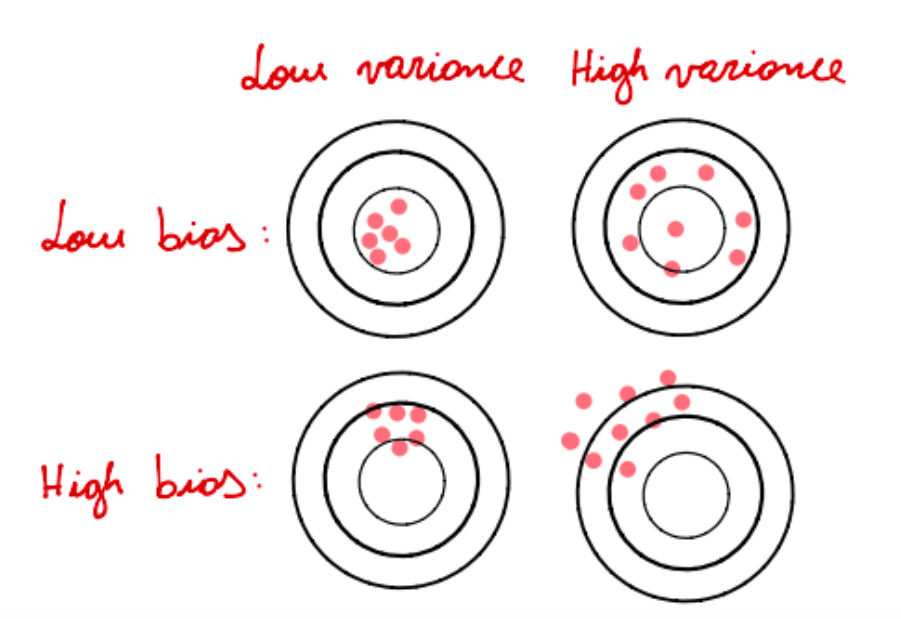
\includegraphics[width=8cm]{bias-variance}
\caption{The effect of bias and variance in the accuracies' prediction.}
\end{figure}\\

\quad \, From the previous explanation of the ordinary least squares method [\ref{chap:Ordinary least squares}], assumes our model $\tilde{z} = \textbf{X}\boldsymbol{\beta}$. \\

The parameters betas can be found by optimizing the means squared error via the so-called cost function: \\

$$C(\boldsymbol{X},\boldsymbol{\beta}) =\frac{1}{n}\sum_{i=0}^{n-1}(z_i-\tilde{z}_i)^2=\mathbb{E}\left[(\boldsymbol{z}-\boldsymbol{\tilde{z}})^2\right]$$ \\

From this, one can prove the bias-variance relationship: \\

\begin{align*}
\label{bias-variance-decomposition}
E[(\boldsymbol{z} - \boldsymbol{\tilde{z}})]^{2} &= E[(f + \epsilon - \boldsymbol{\tilde{z}})]^{2}\\ &= E[(f + \epsilon - \boldsymbol{\tilde{z}} + E[\boldsymbol{\tilde{z}}] - E[\boldsymbol{\tilde{z}}])^{2}]\\ &= E[(f - E[\boldsymbol{\tilde{z}}]^{2})] + E[\epsilon^{2}] + E[E[(\boldsymbol{\tilde{z}} - \boldsymbol{\tilde{z}})^{2}] + 2E[(f - E[\boldsymbol{\tilde{z}}] \epsilon)]\\ &+ 2E[\epsilon(E[\boldsymbol{\tilde{z}}] - \boldsymbol{\tilde{z}})] + 2E[(E[\boldsymbol{\tilde{z}}] - \boldsymbol{\tilde{z}})(f-E[\boldsymbol{\tilde{z}}])]\\ &= (f - E[\boldsymbol{\tilde{z}}])^{2} + E[\epsilon^{2}] + E[(E[\boldsymbol{\tilde{z}}] - \boldsymbol{\tilde{z}})^{2}]\\ &+ 2(f-E[\boldsymbol{\tilde{z}}])E[\epsilon] + 2E[\epsilon]E[E[\boldsymbol{\tilde{z}}]-\boldsymbol{\tilde{z}}] + 2E[E[\boldsymbol{\tilde{z}}]-\boldsymbol{\tilde{z}}](f-E[\boldsymbol{\tilde{z}}])\\ &= (f-E[\boldsymbol{\tilde{z}}]^{2} + E[\epsilon^{2}] + E[(E[\boldsymbol{\tilde{z}}] - \boldsymbol{\tilde{z}})^{2}]\\ &= (f-E[\boldsymbol{\tilde{z}}])^{2} + \sigma^{2} + Var[\boldsymbol{\tilde{z}}]\\ &= Bias(\boldsymbol{\tilde{z}})^{2} + \sigma^{2} + Var(\boldsymbol{\tilde{z}})
\end{align*}\\

\noindent where, \\

\begin{align*}
Var(\textbf{z}) &= E[(\boldsymbol{\tilde{z}} - E[\boldsymbol{\tilde{z}}])^{2}]\\ &= E[(\textbf{y}-f)^{2}]\\ &= E[(f + \epsilon - f)^{2}]\\ &= E[\epsilon^{2}]\\ &= Var[\epsilon] + E[\epsilon]^{2}\\ &= \sigma^{2}
\end{align*}

\noindent and, \\

\begin{align*}
Bias(\boldsymbol{\tilde{z}}) &= E[\boldsymbol{\tilde{z}} - f]\\ &= E[\boldsymbol{\tilde{z}}] - f
\end{align*}
